\documentclass[12pt,a4paper]{article}

% --- Настройка языка и шрифтов для LuaLaTeX ---
\usepackage{fontspec}
\defaultfontfeatures{Ligatures=TeX,Scale=MatchLowercase}
\setmainfont{Alice-Regular}[Path=font/,Extension=.ttf]
\newfontfamily\cyrillicfont{Alice-Regular}[Path=font/,Extension=.ttf]
\usepackage{polyglossia}
\setmainlanguage{russian}
\setsansfont{TeX Gyre Heros}
\setmonofont{TeX Gyre Cursor}

\usepackage{graphicx}        					% Графика
\usepackage[protrusion=false]{microtype}       	% Микротипографика
\usepackage{amsmath, amsfonts, amssymb, amsthm}	% Математика
\usepackage{braket} 							% Braket нотация для квантовой механики
\usepackage{unicode-math} 						% Современный пакет для математики в LuaLaTeX
% \setmathfont{Latin Modern Math} 				% Математический аналог CMU 
\usepackage{longtable}       					% Таблицы с разрывом страниц
\usepackage{tikz}           					% Рисование
\usepackage{circuitikz}       					% Микросхемы
\usepackage{listings}							% Для отображения кода
\usepackage{tabularx}       					% Для таблиц во всю ширину
\usepackage{array}		  						% Для расширенных возможностей таблиц
\usepackage[a4paper,left=20mm,right=20mm,top=20mm,bottom=20mm]{geometry}

% --- Колонтитулы ---
\usepackage{fancyhdr}
\pagestyle{fancy}
\fancyhf{}

\renewcommand{\headrulewidth}{0.4pt}
\renewcommand{\footrulewidth}{0.4pt}
\renewcommand\lstlistingname{Исходный код}

\lstdefinestyle{main}{
	backgroundcolor=\color{gray!8},   
	commentstyle=\color{green!50!black},
	keywordstyle=\color{blue!80!black},
	numberstyle=\small\color{darkgray},
	stringstyle=\rmfamily\color{orange!90!black},
	basicstyle=\ttfamily\small,
	breakatwhitespace=false,         
	breaklines=true,                   
	keepspaces=true,                 
	numbers=left,                    
	numbersep=8pt,                  
	showspaces=false,                
	showstringspaces=false,
	showtabs=false,                  
	tabsize=4
}	

\lstset{style=main}

\title{
	МИНОБРНАУКИ РОССИИ

	федеральное государственное автономное образовательное учреждение

	высшего образования

	«Национальный исследовательский университет
	«Московский институт электронной техники»

	Кафедра КФН
	\vspace{2em}
}
\author{
}
\date{}

\begin{document}

\maketitle
\thispagestyle{fancy}

\begin{center}
\Large Отчёт по Лабораторной работе 2\\
по дисциплине «Квантовая механика»\\
«Свободное движение электрона. Волновой пакет»
\end{center}

\begin{center}
\Large Вариант 1
\end{center}

\vspace{12em}

\begin{table}[h]
\noindent
\begin{tabular*}{\textwidth}{@{\extracolsep{\fill}} p{0.48\textwidth} p{0.52\textwidth}}
Студент, группа & Андреев Иван Алексеевич, ЭН-$25$ \\
[0.5em] Руководитель & Журавлёв Максим Николаевич
\end{tabular*}
\end{table}

\cfoot{Москва 2026}

\pagebreak

\fancyhead[L]{Задание 1} 
\fancyhead[R]{Квантовая механика}
\fancyfoot[C]{\thepage}

\begin{center}
	\textbf{\LARGE Задание 1}
\end{center}

Согласно варианту были взяты параметры $E_0=20$ эВ и $d_0=1$ Å. Параметры подобраные 
для наглядного отображения волнового пакета $\psi(x,t)$ представлены 
ниже.

\begin{lstlisting}[language=Matlab, firstnumber=12, 
	title={\textbf{free\_movement.m}}]
m = 9.1e-31;                % mass of electron (kg)
h = 1.05e-34;               % Plank's constant (J*s)
E0 = 20;                    % energy of electron (eV)
v0 = sqrt(2*E0*1.6e-19/m);  % velocity of electron (m/s)
d0 = 1;                     % half-width of wave packet (A, Angstroem)
x0 = 10.0;                  % center of wave packet (A, Angstroem)

%-------------------------------------------------------------
% TINE AND SPACE PARAMETERS

% time points, (fs, femtosecond)
t0 = 0;
t1 = 0.1;       
t2 = 0.2;
t3 = 0.3;
t4 = 0.4;

% begin and end of line segment of axis 'x'
xBegin = 5;
xEnd = 35;
\end{lstlisting}

График полученный в результате выполнения кода из файла \textbf{free\_movement.m} 
представлен на Рис.~\ref{fig:lab2qmTask1}.

\begin{figure}[h]
\centering
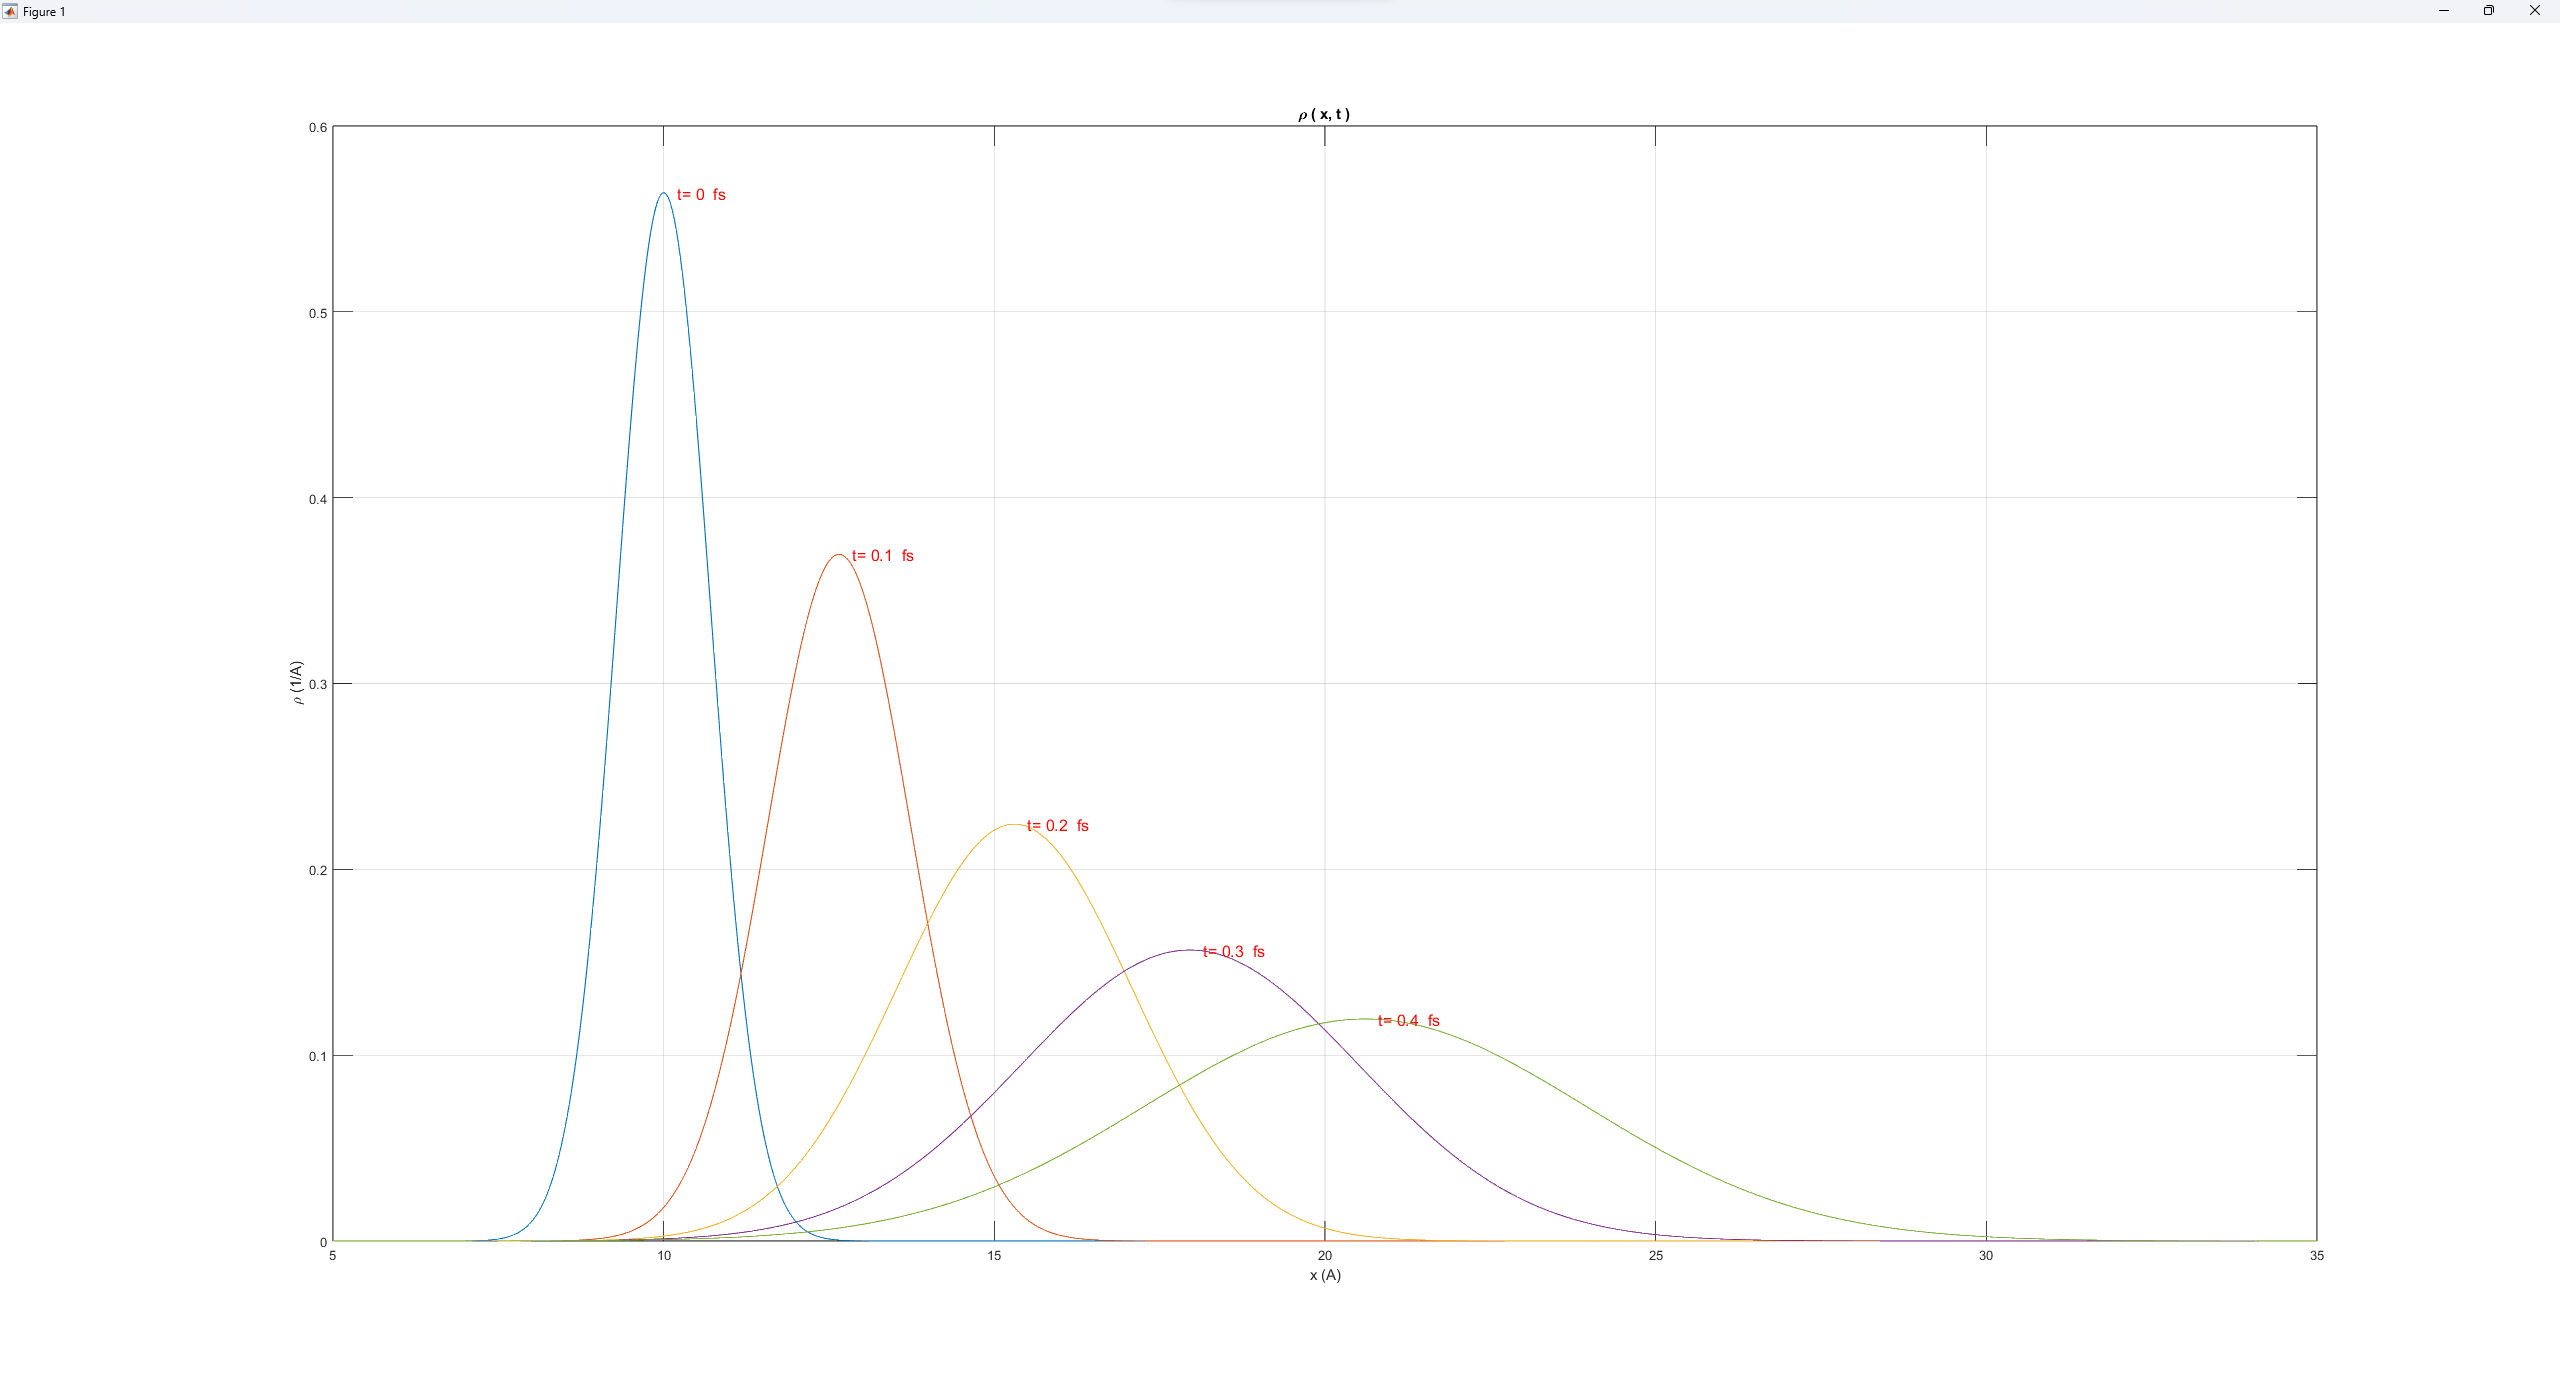
\includegraphics[width=\textwidth]{Lab2qmTask1.png}
\caption{График волнового пакета $\psi(x,t)$ с параметрами $E_0=20$ эВ и $d_0=1$ Å.}
\label{fig:lab2qmTask1}
\end{figure}

Масса электрона $m_{e^-} = 9.10938356 \times 10^{-31}$ кг, энергия электрона $E_0 = 20$ эВ, 
уравнение связывающее энергию и импульс:
\begin{equation}
	E_0 = \frac{p_0^2}{2m_{e^-}} \Longrightarrow p_0 = \sqrt{2m_{e^-}E_0}
\end{equation}

Импуль электрона $p_0$ в свою очередь связан со скоростью $v_0$ следующим образом:
\begin{equation}
	v_0 = \frac{p_0}{m_{e^-}} = \sqrt{\frac{2E_0}{m_{e^-}}}
	\label{eq:velocity}
\end{equation}

Из формулы (\ref{eq:velocity}) найдём скорость электрона $v_0$:
\begin{equation*}
	v_0 = \sqrt{\frac{2E_0}{m_{e^-}}}= \sqrt{\frac{2\cdot 20\cdot 1.6\cdot 10^{-19}}{9.10938356 \cdot 10^{-31}}} \approx 26.506 \text{ Å/фс}
\end{equation*}

\begin{center}
	\textbf{\LARGE Задание 2}
\end{center}

\fancyhead[L]{Задание 2} 

В первую очередь необходимо определить дескрипторы полу-ширины волнового пакета $d$ 
по аналогии с предыдущими дескрипторами,
первый отвечает за отображение статичного текста пояснения, второй — за отображение 
самого значения полу-ширины.

\begin{lstlisting}[language=Matlab, firstnumber=83, 
	title={\textbf{Work\_Window.m}}]
% create contol - text
hTxtys3T = uicontrol(hFig1, "Style","text", ...
    "String",'d (t) = ', ...
    'Units','normalized', ...
    'Position',[0.7 0.93 0.1 0.05], ...
    'Visible', 'off', ...
    'BackgroundColor',[0.8 0.7 0.7]);

% create control - text
hTxtys3 = uicontrol(hFig1, "Style","text", ...
    "String",'0', ...
    'Units','normalized', ...
    'Position',[0.8 0.93 0.1 0.05], ...
    'Visible', 'off', ...
    'BackgroundColor',[0.8 0.7 0.7]);
\end{lstlisting}

Также доопределим в глобальные перменные новые текстовые дескрипторы.

\begin{lstlisting}[language=Matlab, firstnumber=4, 
	title={\textbf{Work\_Window.m}}]
% handle of figure
global hFig1;
% handles of contrles 'pushbutton'
global hBut1 hBut2 hBut3 hBut4 ;
% handles of contrles 'text'
global hTxtys1 hTxtys1T hTxtys2 hTxtys2T hTxtys3 hTxtys3T;
\end{lstlisting}

Доопределим также и для файла содержащего основной цикл исполнения \textbf{Move\_Packet.m}.

\begin{lstlisting}[language=Matlab, firstnumber=6, 
	title={\textbf{Move\_Packet.m}}]
% handle of figure
global hFig1;
% handles of contrles 'pushbutton'
global hBut1 hBut2 hBut3 hBut4;
% handles of contrles 'text'
global hTxtys1 hTxtys1T hTxtys2 hTxtys2T hTxtys3 hTxtys3T;
\end{lstlisting}

Определим дескрипторы как видмые.

\begin{lstlisting}[language=Matlab, firstnumber=13, 
	title={\textbf{Move\_Packet.m}}]
% set for controls next mode: 'Enable off' or 'Enable on'
set(hBut1,'Visible','on','Enable','off');
set(hBut2,'Visible','on','Enable','on');
set(hBut4,'Visible','on','Enable','on');

set(hTxtys1,'Visible','on','Enable','on');
set(hTxtys1T,'Visible','on','Enable','on');
set(hTxtys2,'Visible','on','Enable','on');
set(hTxtys2T,'Visible','on','Enable','on');
set(hTxtys3,'Visible','on','Enable','on');
set(hTxtys3T,'Visible','on','Enable','on');
\end{lstlisting}

Внутри основного цикла исполнения определим обновление значения дескприптора значения
полу-ширины волнового пакета $d$.

\begin{lstlisting}[language=Matlab, firstnumber=102, 
	title={\textbf{Move\_Packet.m}}]
	% print of half-width of wave packet
    str = num2str(dFun(h,m,d0,t));
    set(hTxtys3,'String',str);
\end{lstlisting}

Итоговый результат представлен на Рис.~\ref{fig:lab2qmTask2part1}.

\begin{figure}[h]
\centering
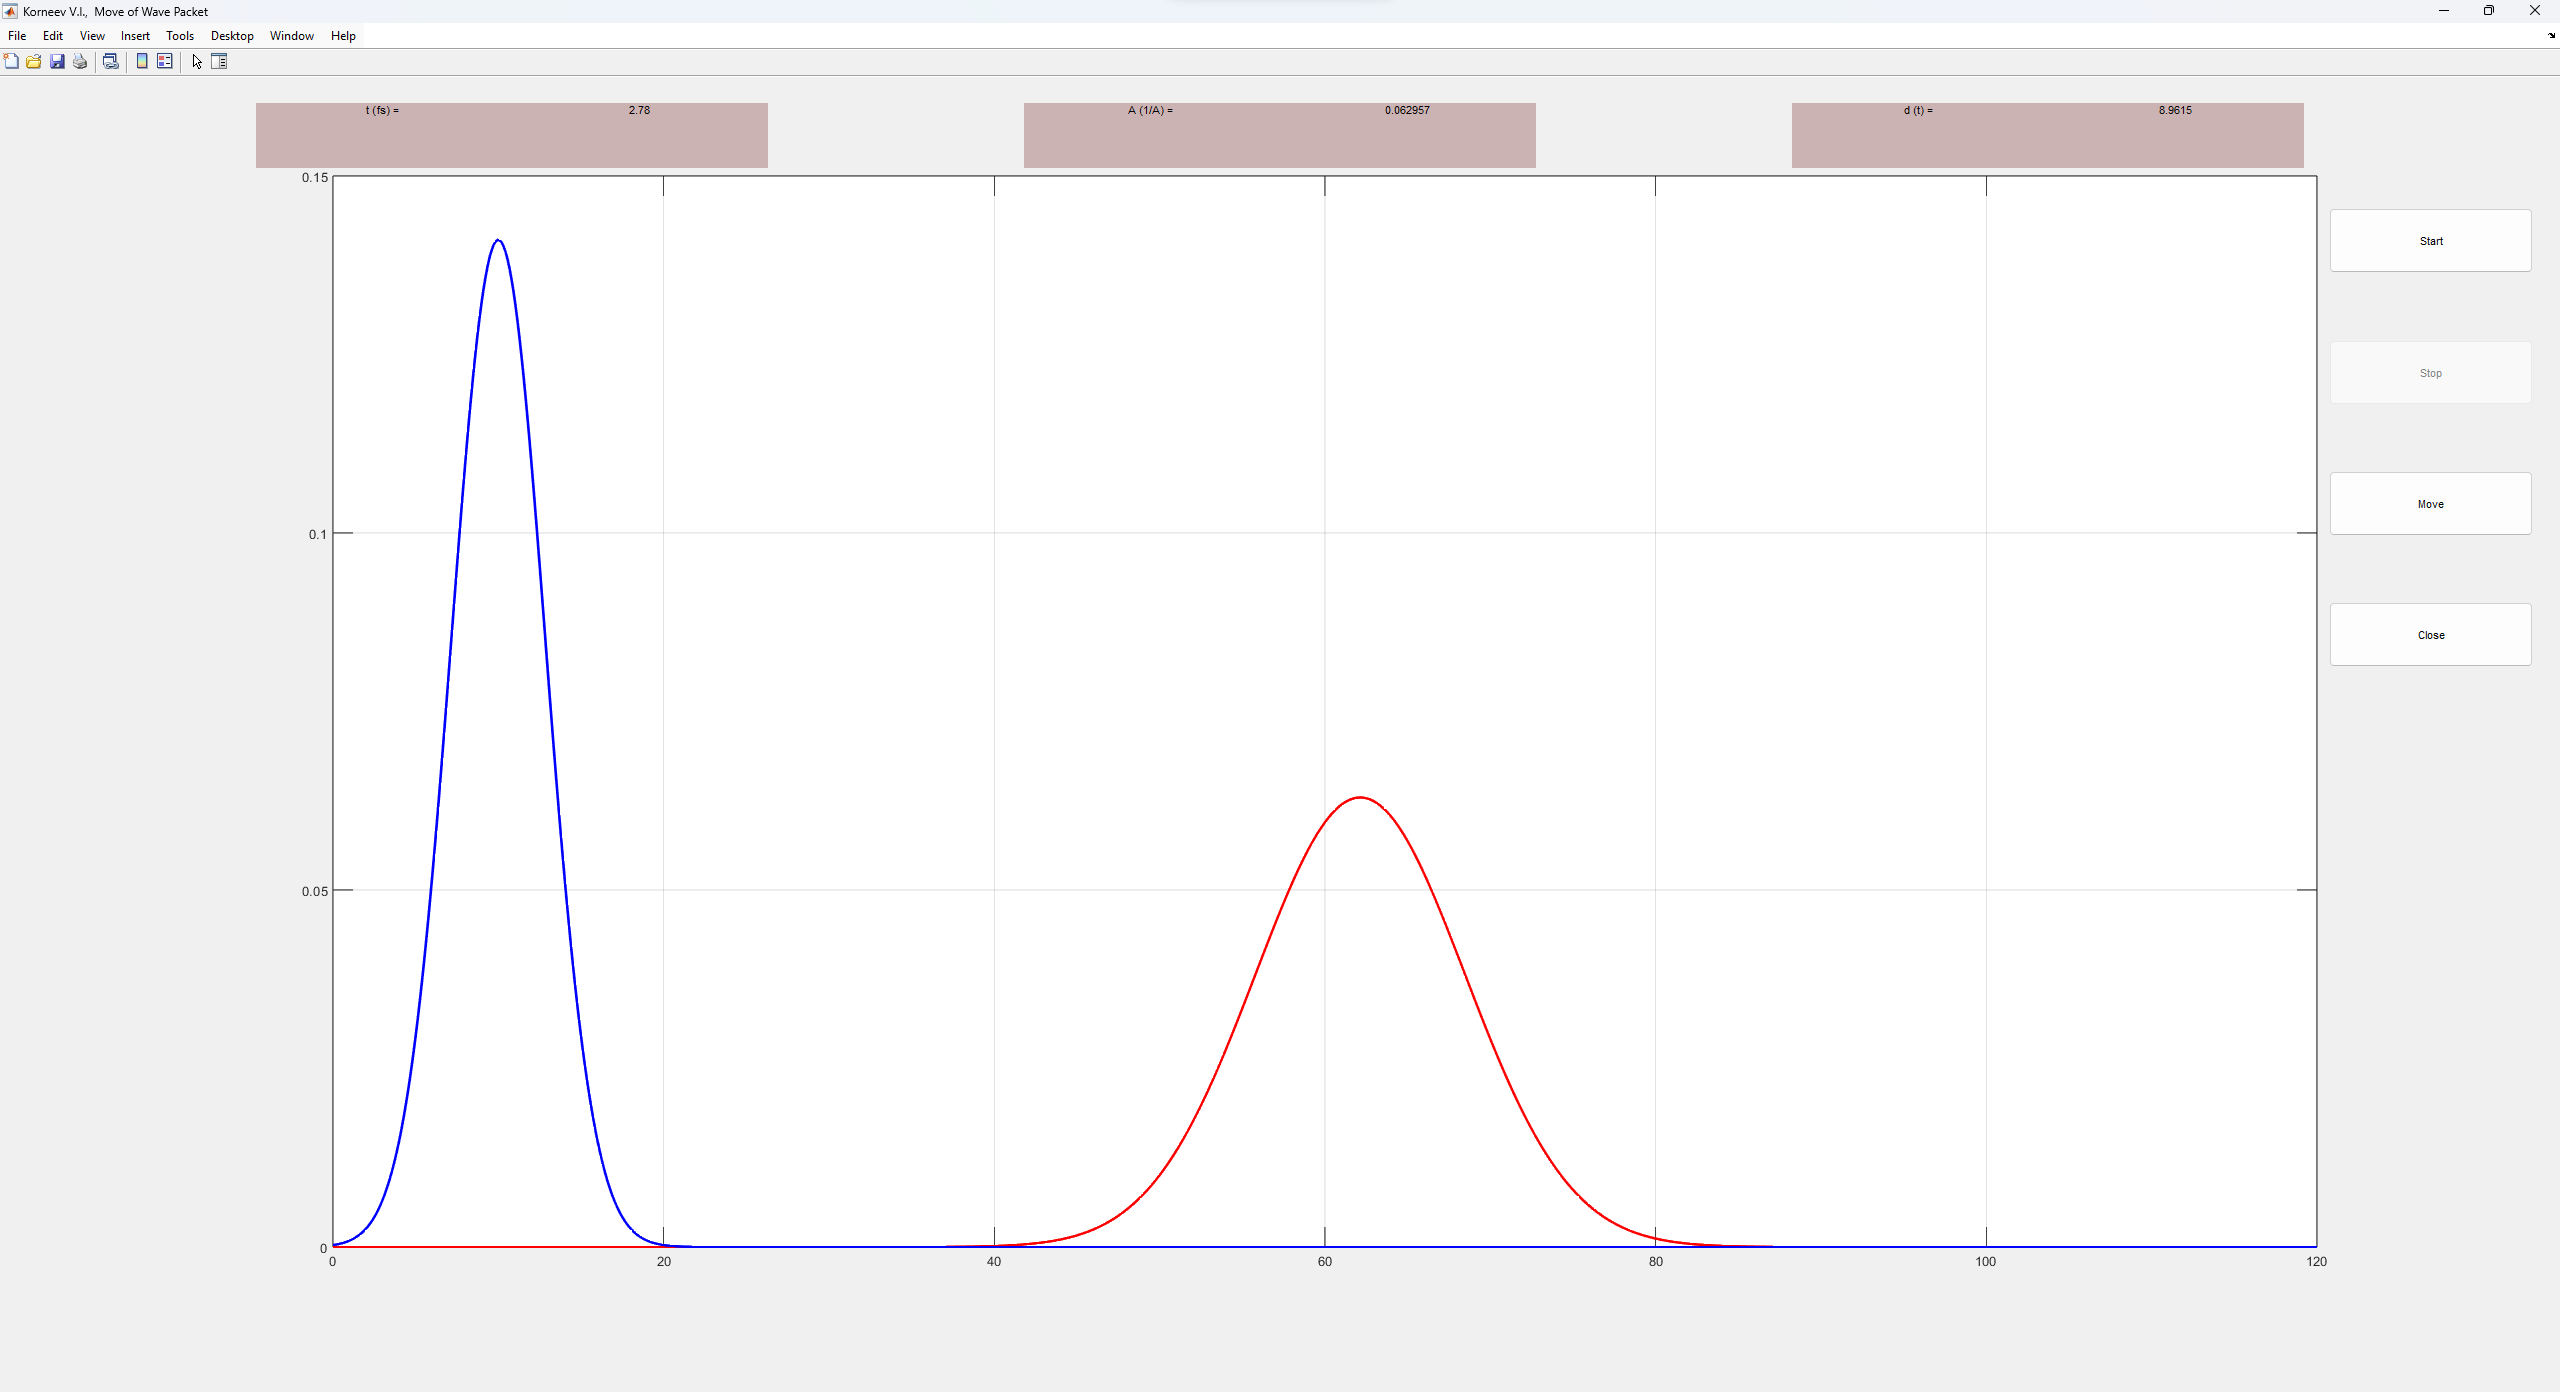
\includegraphics[width=\textwidth]{Lab2qmTask2part1.png}
\caption{График волнового пакета $\psi(x,t)$ с отображением значения 
полу-ширины $d$ в реальном времени, идентичный примерному.}
\label{fig:lab2qmTask2part1}
\end{figure}

Подставим значения $E_0=20$ эВ и $d_0=1$ Å согласно варианту.

\begin{lstlisting}[language=Matlab, firstnumber=30, 
	title={\textbf{Move\_Packet.m}}]
%-------------------------------------------------------------
% PARAMETERS OF TASK

m = 9.1e-31;                %mass of electron (kg)
h = 1.05e-34;               %Plank's constant (J*s)
E0 = 20;                    %energy of electron (eV)
v0 = sqrt(2*E0*1.6e-19/m);  %velocity of electron (m/s)
d0 = 1;                     %half-width of wave packet (A, Angstroem)
x0 = 10.0;                  %center of wave packet (A, Angstroem)
\end{lstlisting}

Также нетрудно понять, что так как $d_0$ в разы ниже изначального значения, то и плотность
вероятности будет куда более локализованной, соотвественно и её пик будет куда выше, что 
требует доопределить границы по оси значений для корректного отображения графика. 

\begin{lstlisting}[language=Matlab, firstnumber=48, 
	title={\textbf{Move\_Packet.m}}]
% begin and end of line segment of axis 'y'
yBottom = 0;
yTop = 0.6;
\end{lstlisting}

Результат выполнения окончальной программы представлен на Рис.~\ref{fig:lab2qmTask2part2}.

\begin{figure}[h]
\centering
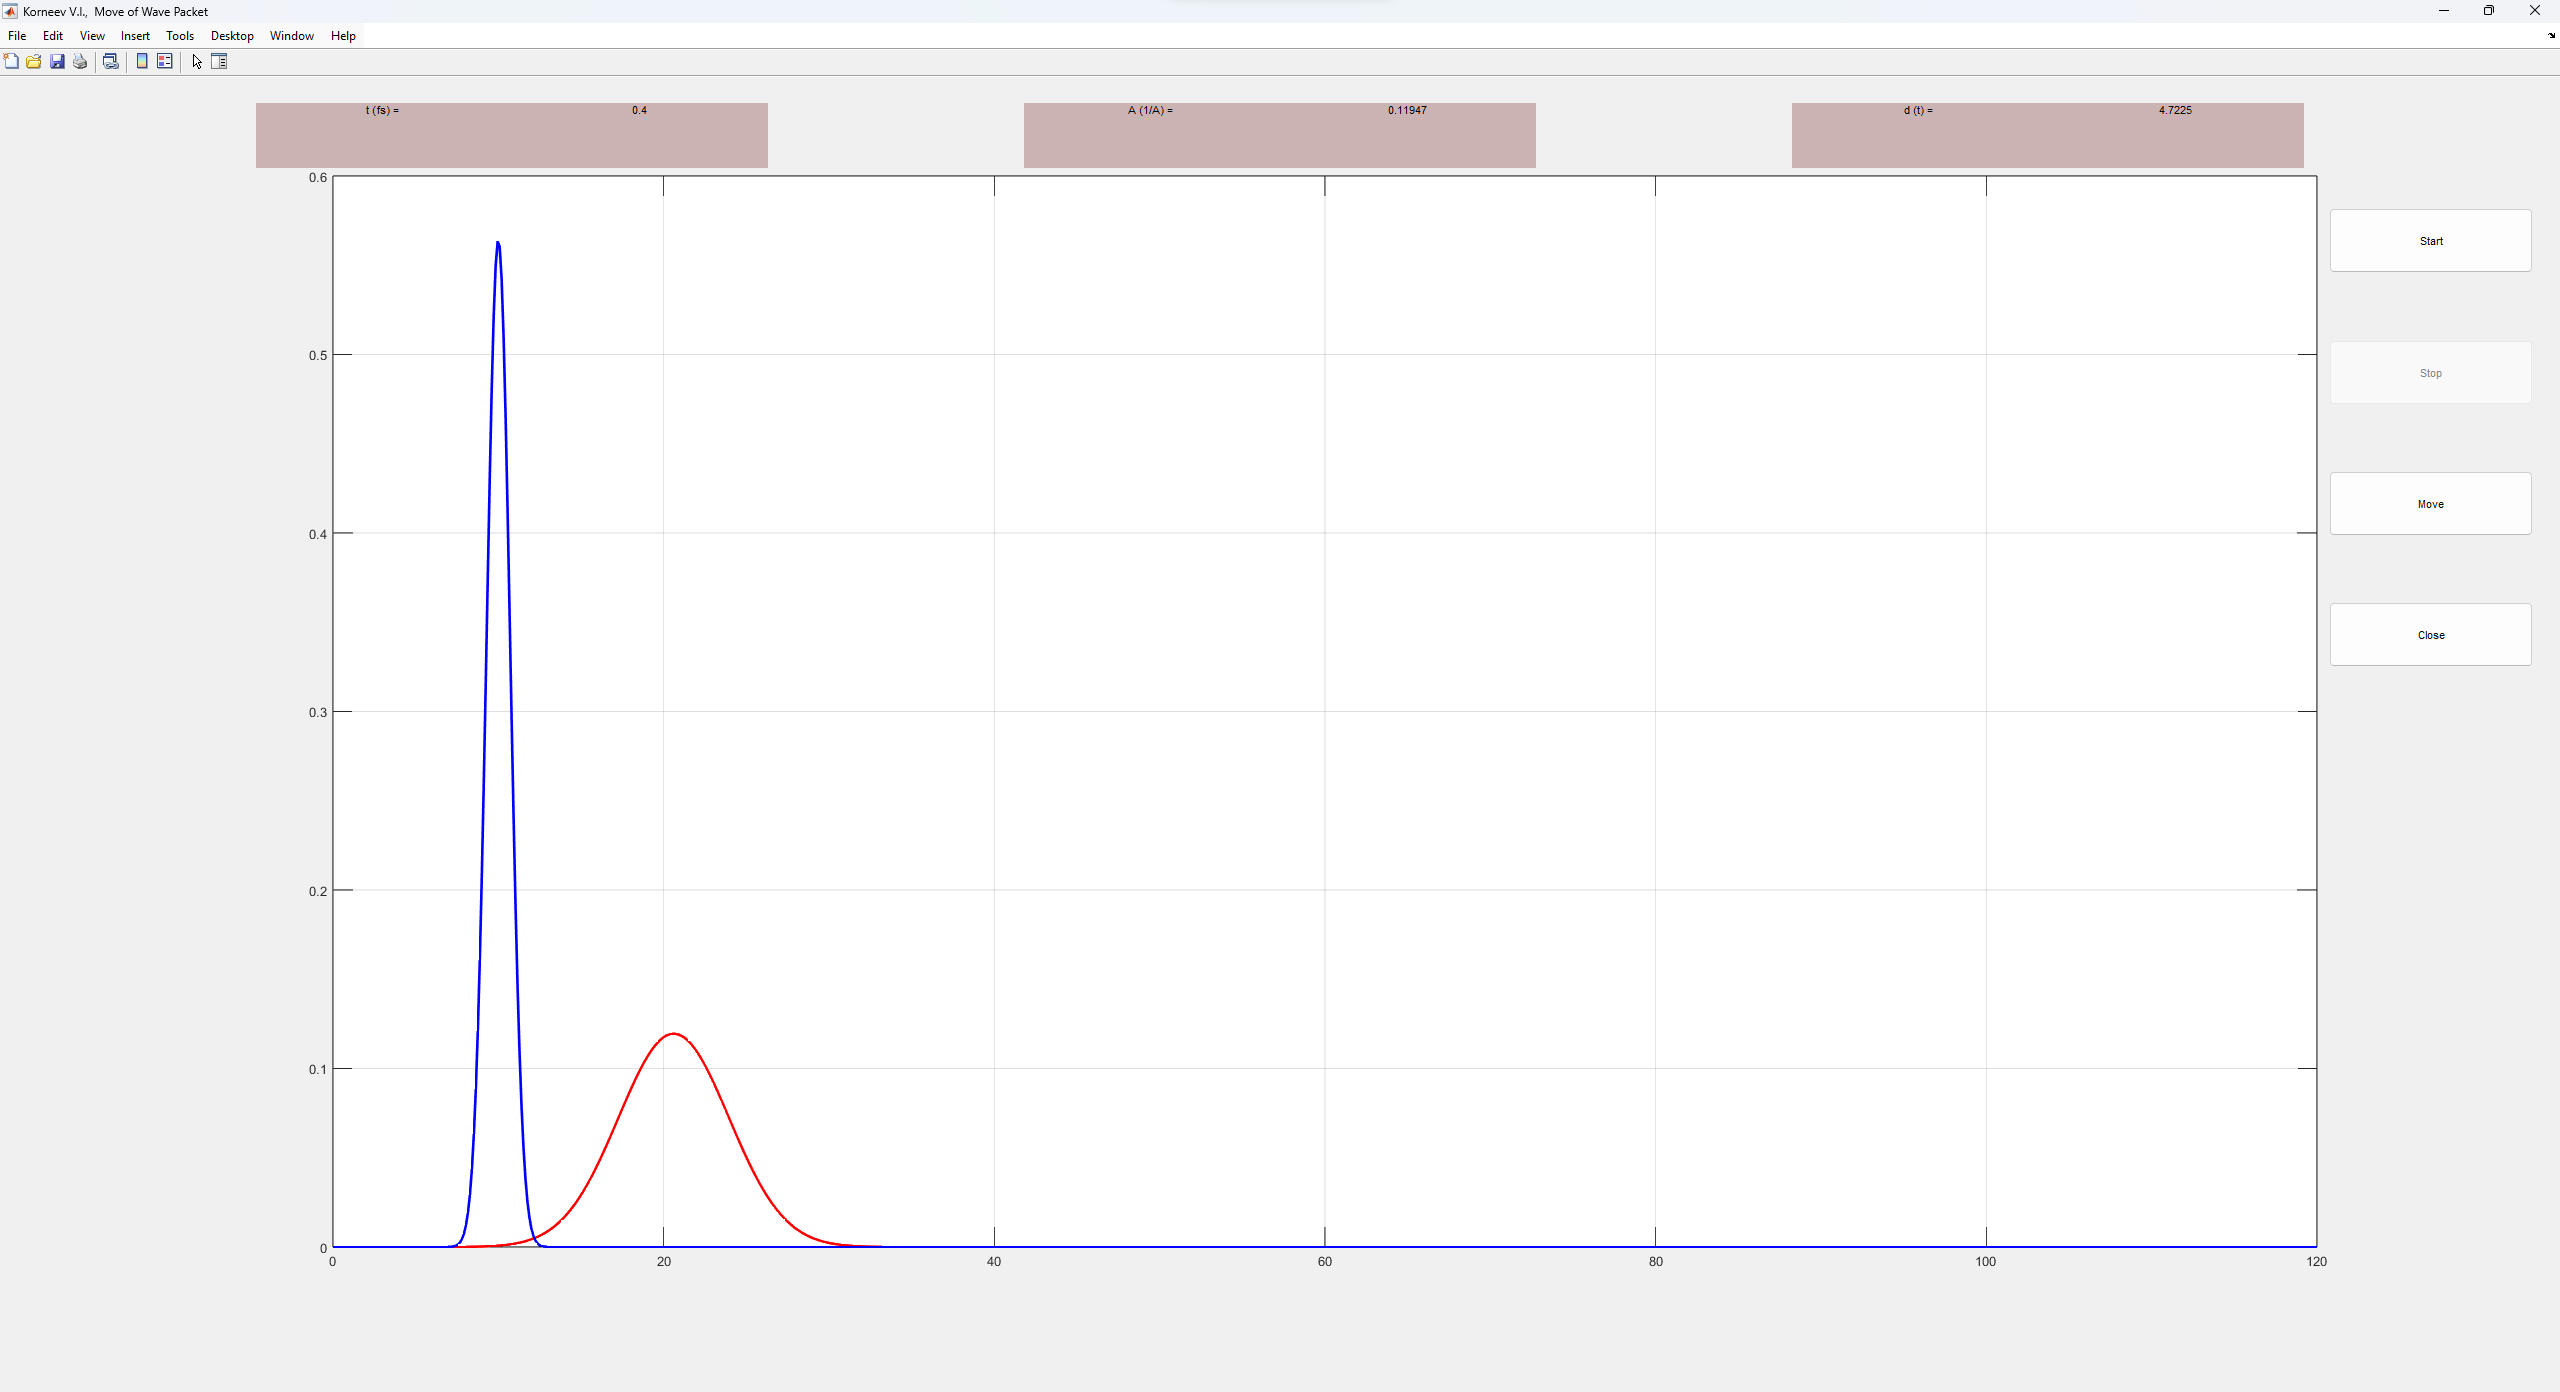
\includegraphics[width=\textwidth]{Lab2qmTask2part2.png}
\caption{График волнового пакета $\psi(x,t)$ с отображением значения 
полу-ширины $d$ в реальном времени для заданных параметров.}
\label{fig:lab2qmTask2part2}
\end{figure}

\begin{center}
	\begin{table}[h]
		\noindent
		\begin{tabularx}{\textwidth}{|>{\centering\arraybackslash}X|>{\centering\arraybackslash}X|>{\centering\arraybackslash}X|>{\centering\arraybackslash}X|>{\centering\arraybackslash}X|>{\centering\arraybackslash}X|}
		\hline
		 & 1 & 2 & 3 & 4 & 5 \\
		\hline
		$t$, фс & 0.2165 & 0.411 & 0.611 & 0.808 & 1.2075 \\
		\hline
		$A$, Å$^{-1}$ & 0.20967 & 0.11641 & 0.079234 & 0.06017 & 0.04039 \\
		\hline
		$d$, Å & 2.6908 & 4.8466 & 7.1206 & 9.3766 & 13.9685 \\
		\hline
		\end{tabularx}
		\caption{Результаты моделирования для $E_0 = 20$ эВ и $d_0 = 1$ Å.}
		\label{tab:lab2qmTask2}
	\end{table}
\end{center}

\pagebreak

\begin{center}
	\textbf{\LARGE Задание 3}
\end{center}

\fancyhead[L]{Задание 3} 

Доопределяем параметры построения для $d_0 = 1$ Å.

\begin{lstlisting}[language=Matlab, firstnumber=7, 
	title={\textbf{amplitude.m}}]
%-------------------------------------------------------------
% PARAMETERS OF TASK

m = 9.1e-31;            %mass of electron (kg)
h = 1.05e-34;           %Plank's constant (J*s)
d0 = 1;                 %half-width of wave packet (A, Angstroem)
\end{lstlisting}

Доопределяем границы по осям для удобоворимого отображения графика.
\begin{lstlisting}[language=Matlab, firstnumber=14, 
	title={\textbf{amplitude.m}}]
% begin and end of line segment of axis 't'
tBegin = 0;
tEnd = 2;
% step along axis 't'
dt = (tEnd - tBegin)/1000; 
% begin and end of line segment of axis 'A'
ABottom = 0;
ATop = 0.6;
\end{lstlisting}

Вносим значения из Таблицы \ref{tab:lab2qmTask2} в код.

\begin{lstlisting}[language=Matlab, firstnumber=23, 
	title={\textbf{amplitude.m}}]
% data from program Wave_Packet
tm = [0.2165 0.411 0.611 0.808 1.2075] 
Am = [0.20967 0.11641 0.079234 0.06017 0.04039] 
\end{lstlisting}

\begin{figure}[h]
\centering
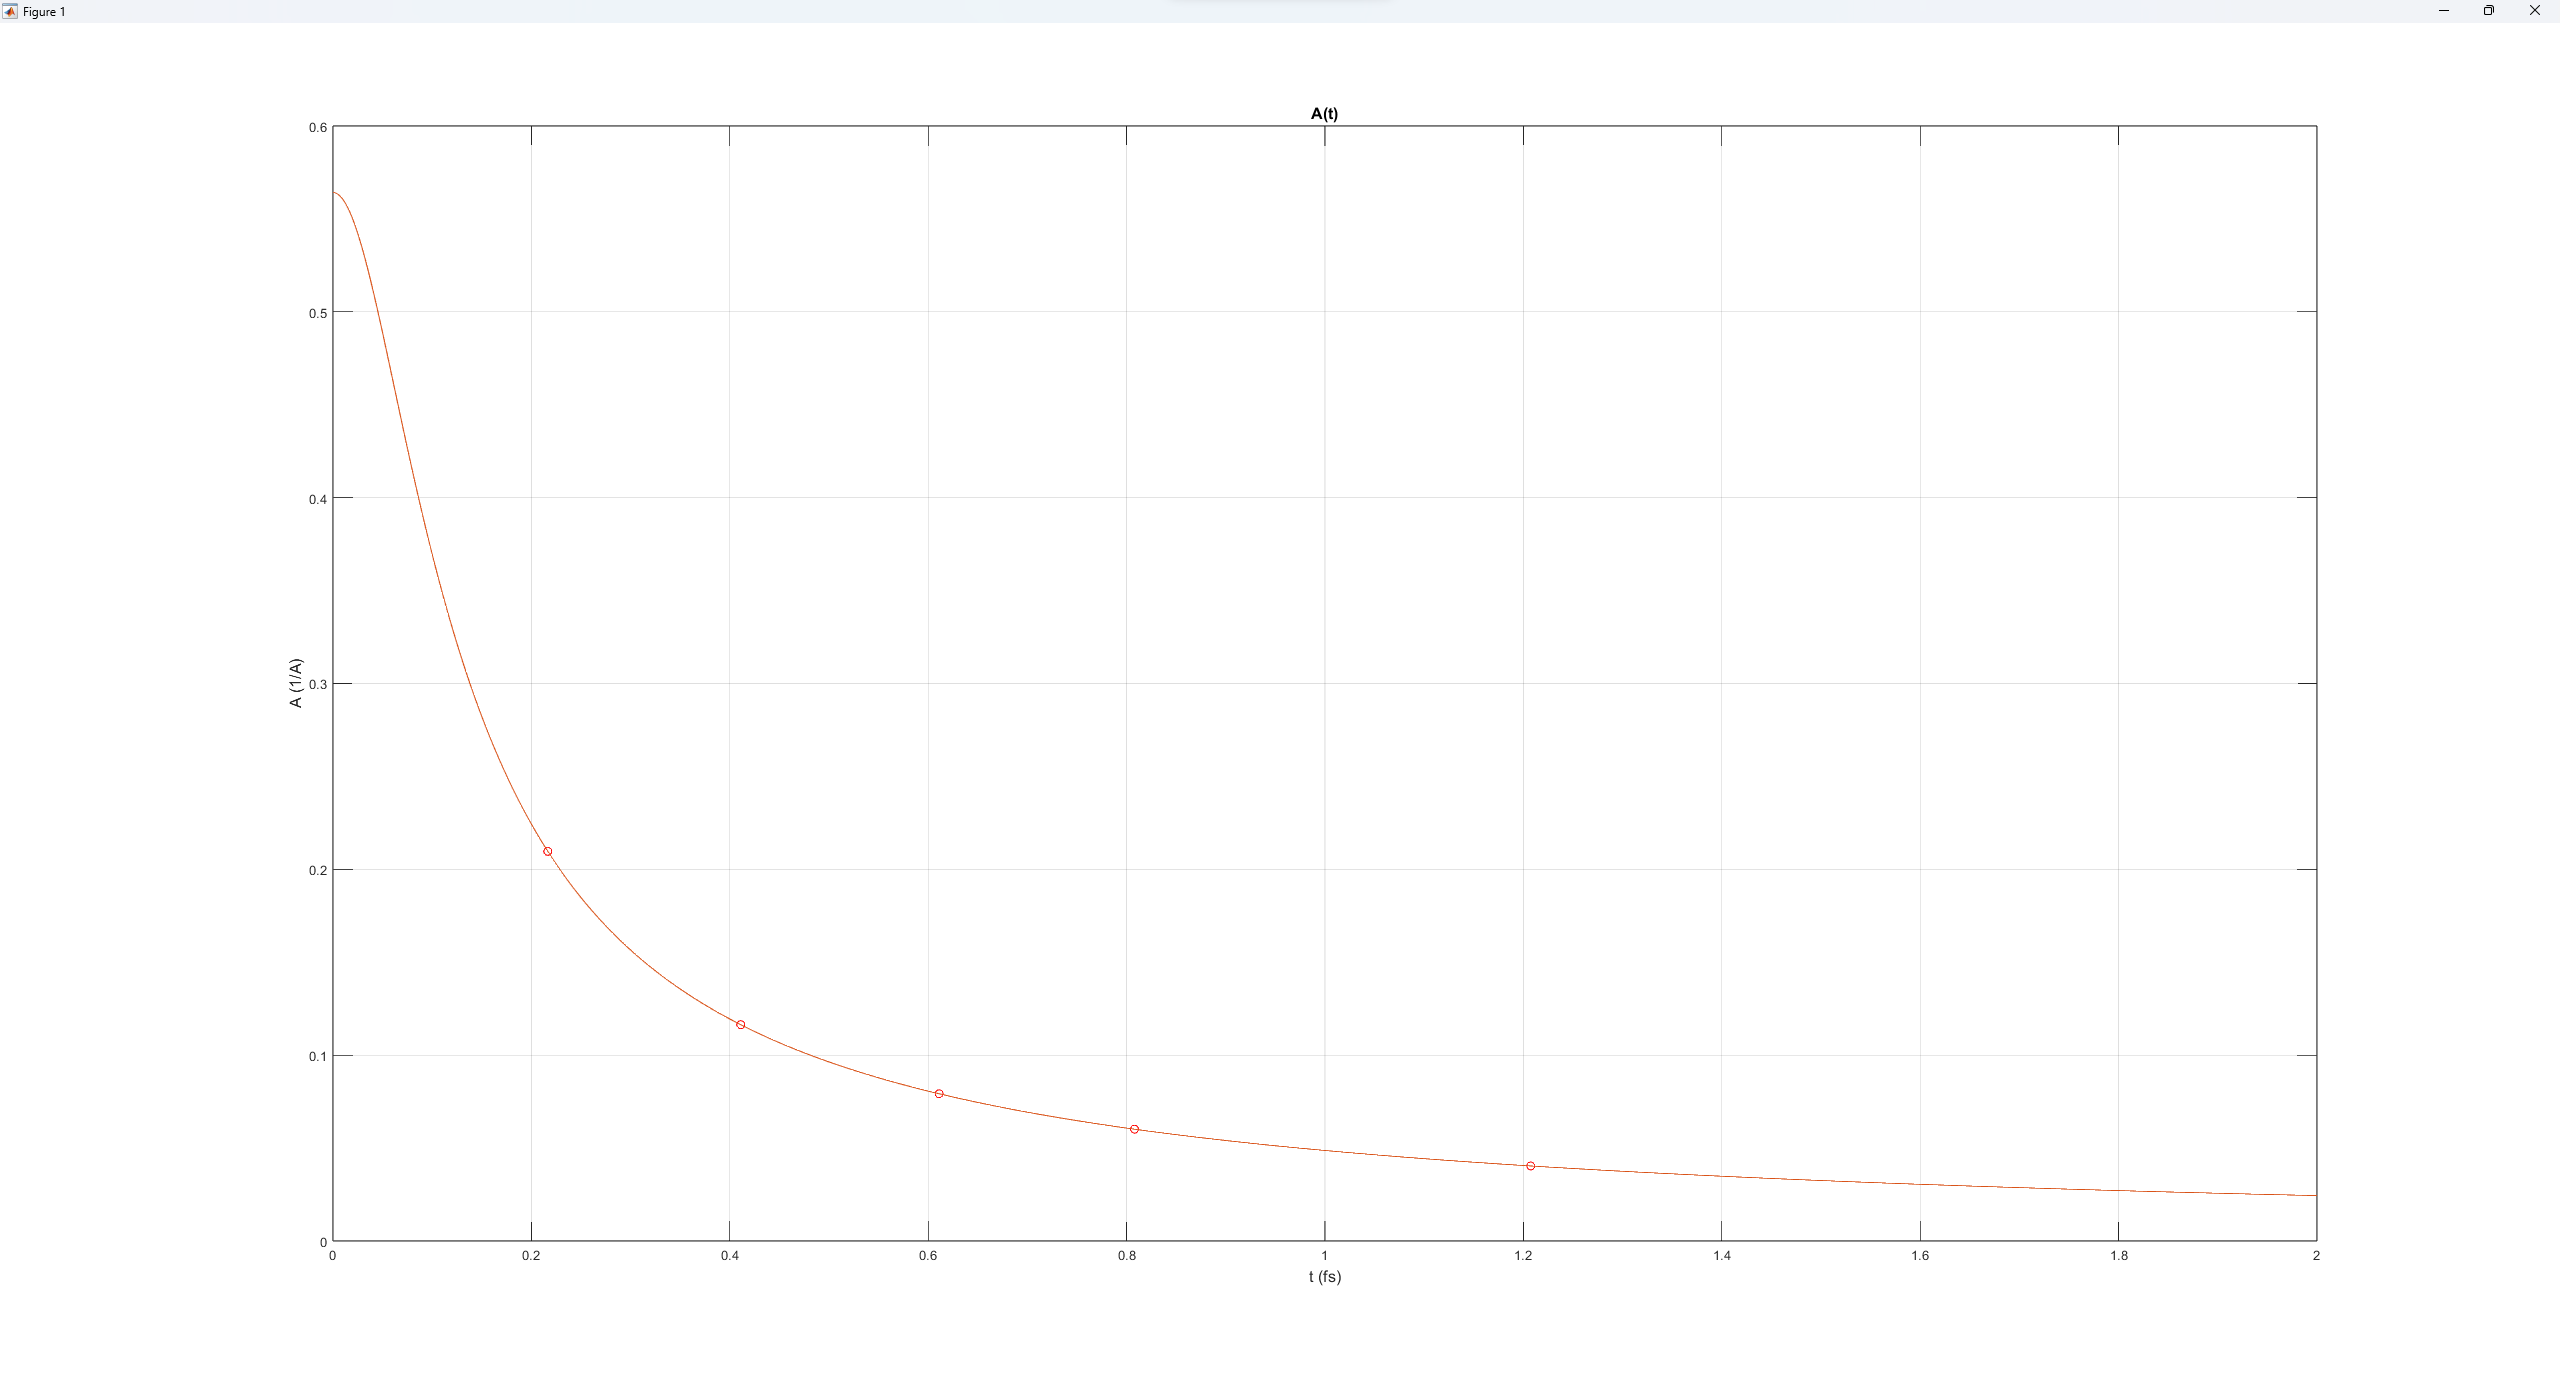
\includegraphics[width=\textwidth]{Lab2qmTask3.png}
\caption{График амплитуды волнового пакета $A(t)$ для $E_0 = 20$ эВ и $d_0 = 1$ Å с 
ключевыми точками из Таблицы \ref{tab:lab2qmTask2}.}
\label{fig:lab2qmTask3}
\end{figure}

\pagebreak

\begin{center}
	\textbf{\LARGE Задание 4}
\end{center}

\fancyhead[L]{Задание 4} 

Доопределяем параметры построения для $d_0 = 1$ Å.

\begin{lstlisting}[language=Matlab, firstnumber=7, 
	title={\textbf{half\_width.m}}]
%-------------------------------------------------------------
% PARAMETERS OF TASK

m = 9.1e-31;            %mass of electron (kg)
h = 1.05e-34;           %Plank's constant (J*s)
d0 = 1;                 %half-width of wave packet (A, Angstroem)
\end{lstlisting}

Доопределяем границы по осям для удобоворимого отображения графика.

\begin{lstlisting}[language=Matlab, firstnumber=14, 
	title={\textbf{half\_width.m}}]
% begin and end of line segment of axis 't'
tBegin = 0;
tEnd = 2;
% step along axis 't'
dt = (tEnd - tBegin)/1000; 
% begin and end of line segment of axis 'A'
ABottom = 0;
ATop = 15;
\end{lstlisting}

Вносим значения из Таблицы \ref{tab:lab2qmTask2} в код.

\begin{lstlisting}[language=Matlab, firstnumber=23, 
	title={\textbf{half\_width.m}}]
% data from program Wave_Packet
tm = [0.2165 0.411 0.611 0.808 1.2075] 
dm = [2.6908 4.8466 7.1206 9.3766 13.9685] 
\end{lstlisting}

\begin{figure}[h]
\centering
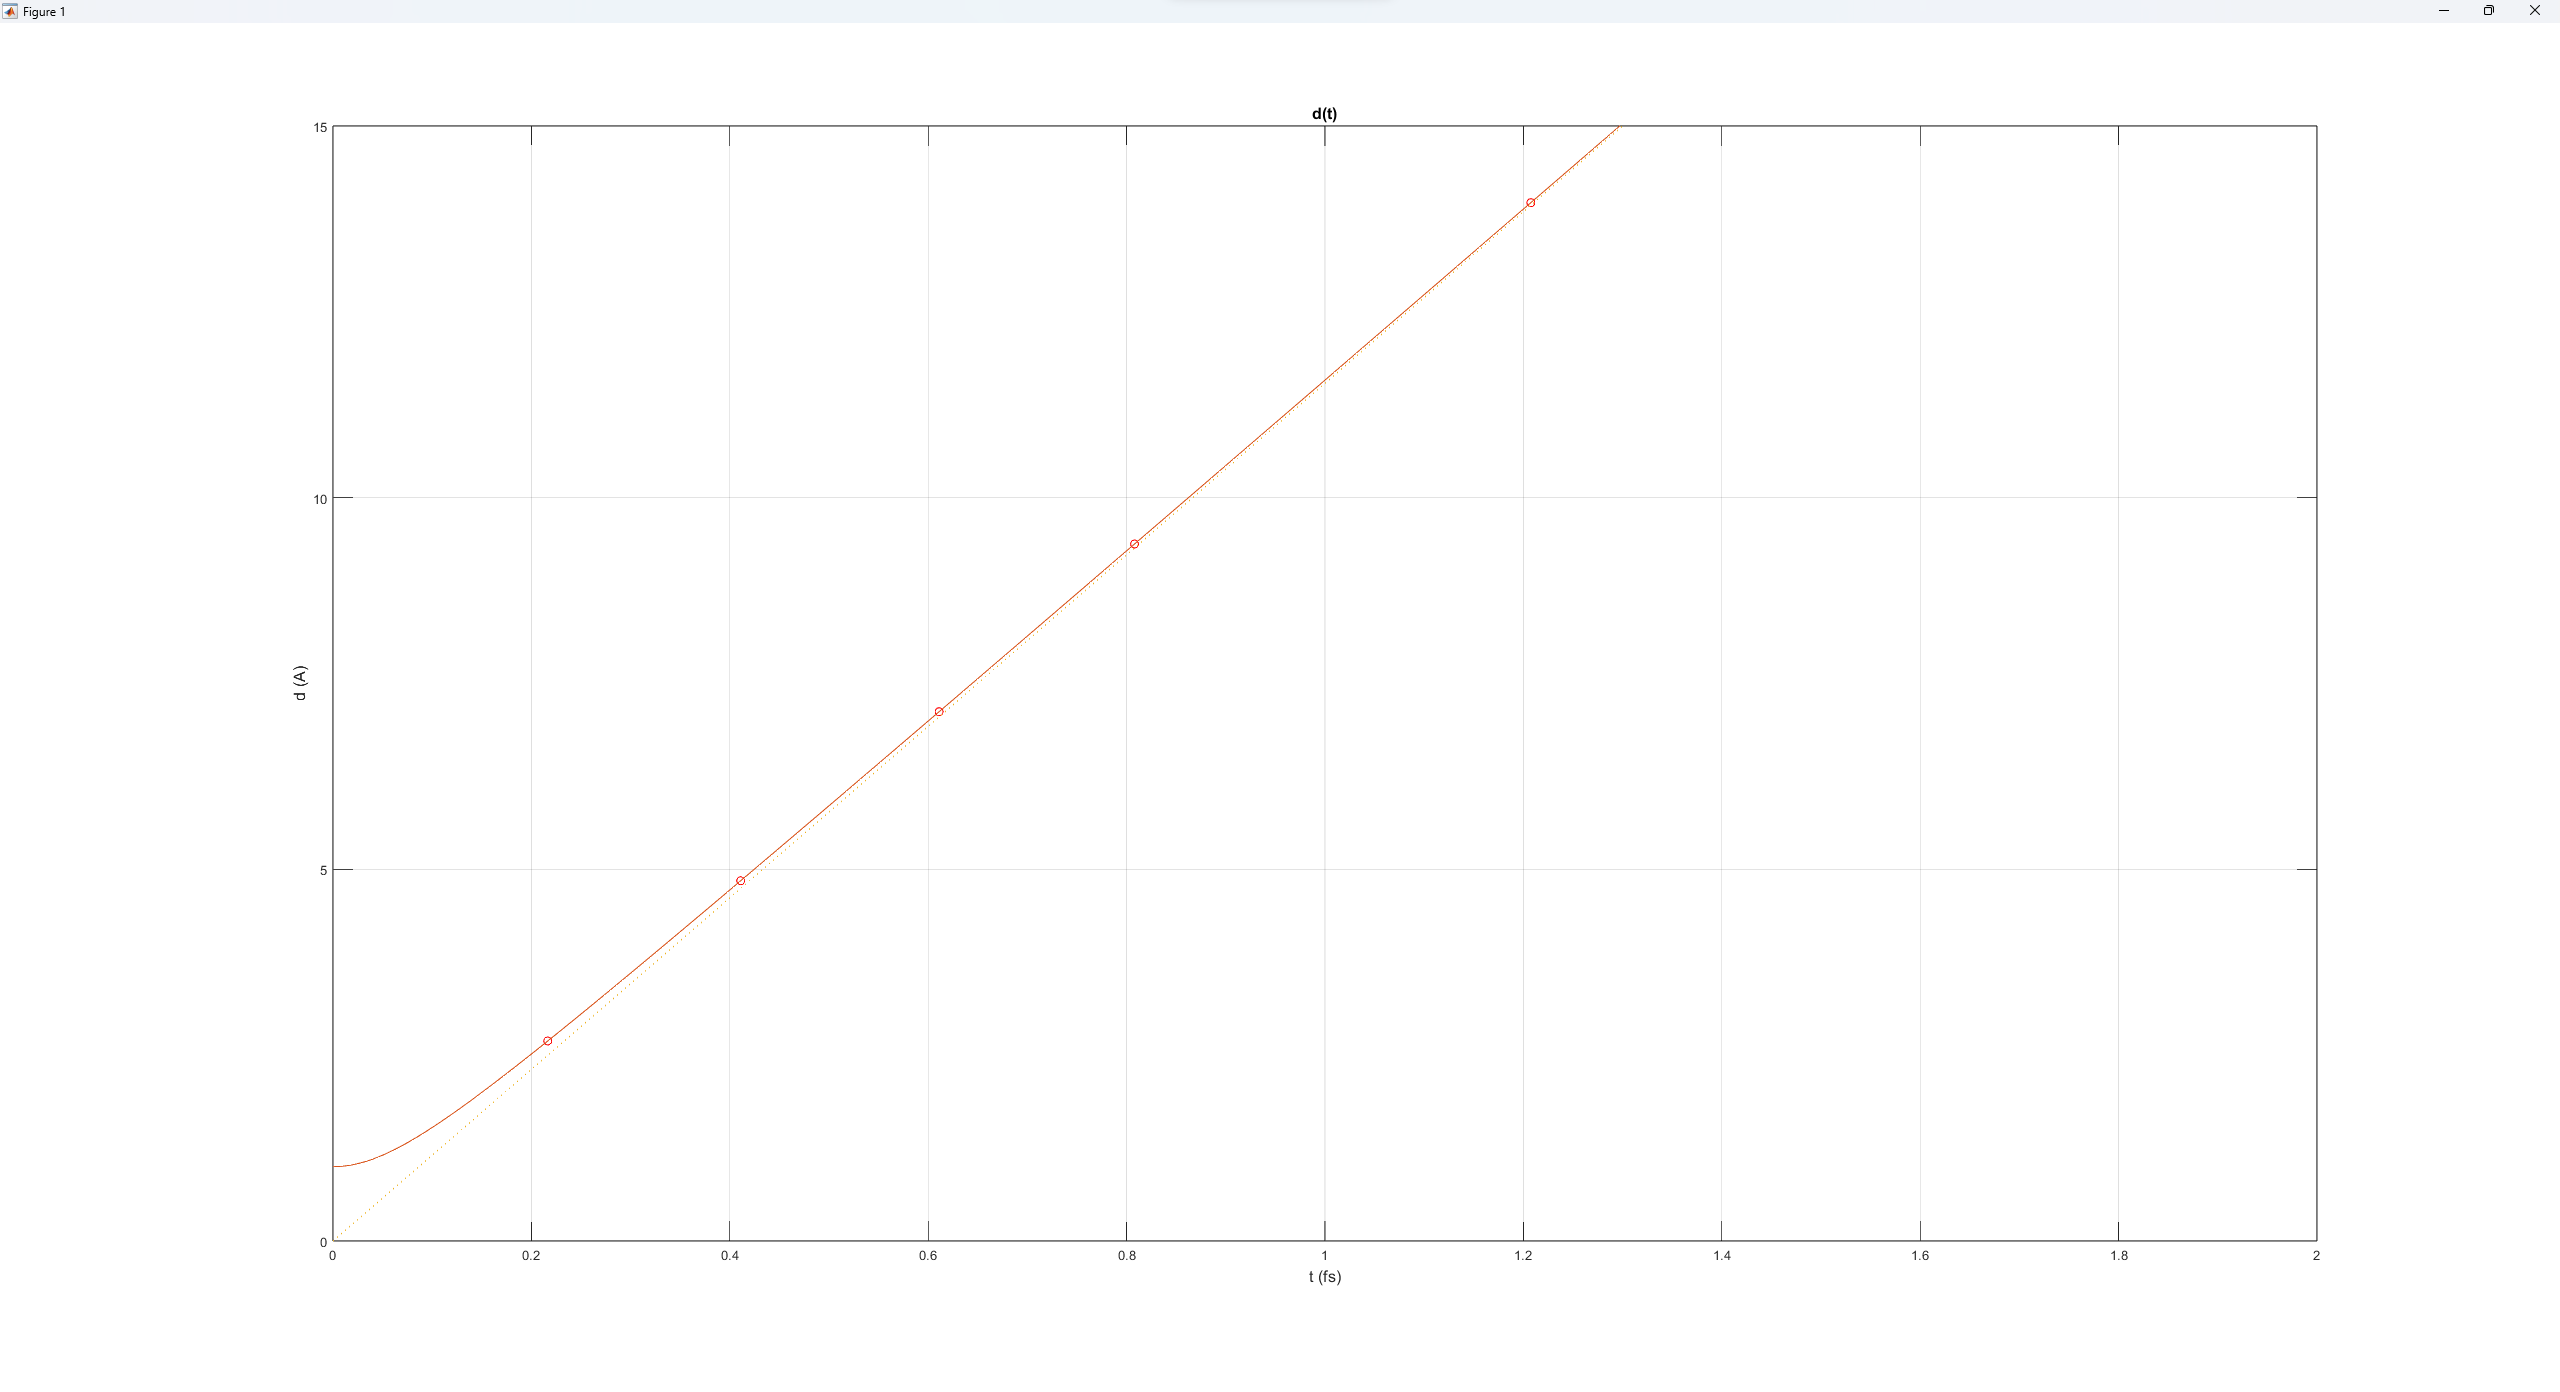
\includegraphics[width=\textwidth]{Lab2qmTask4.png}
\caption{График полу-ширины волнового пакета $d(t)$ для $E_0 = 20$ эВ и $d_0 = 1$ Å с ключевыми точками из Таблицы \ref{tab:lab2qmTask2}.}
\label{fig:lab2qmTask4}
\end{figure}

\pagebreak

\begin{center}
	\textbf{\LARGE Задание 5}
\end{center}

\fancyhead[L]{Задание 5} 

Доопределяем параметры построения для $E_0 = 20$ эВ и $d_0 = 1$ Å.

\begin{lstlisting}[language=Matlab, firstnumber=6, 
	title={\textbf{momentum\_distribution.m}}]
%-------------------------------------------------------------
% PARAMETERS OF TASK

m = 9.1e-31;                % mass of electron (kg)
h = 1.05e-34;               % Plank's constant (J*s)
E0 = 20;                    % energy of electron (eV)
d0 = 1;                     % half-width of wave packet (A, Angstroem)
\end{lstlisting}

Доопределяем границы по осям для удобоворимого отображения графика.

\begin{lstlisting}[language=Matlab, firstnumber=20, 
	title={\textbf{momentum\_distribution.m}}]
% begin and end of line segment of axis 'p'
pBegin = 0;
pEnd = 50;
% step along axis 'p'
dp = (pEnd - pBegin)/1000; 
% begin and end of line segment of axis 'Ro'
RoBottom = 0;
RoTop = 0.08;
\end{lstlisting}

На Рис.~\ref{fig:lab2qmTask5} представлен график распределения вероятности по импульсам 
$\rho(p)$ для $E_0 = 20$ эВ и $d_0 = 1$ Å, построенный на основе кода из файла 
\textbf{momentum\_distribution.m}. Зелённая вертикальная линия соответствует импульсу $p_0$, рассчитанному по формуле
\begin{equation}
	p_0 = \sqrt{2m_{e^-}E_0}
	\label{eq:impulse}
\end{equation}
\begin{figure}[h]
\centering
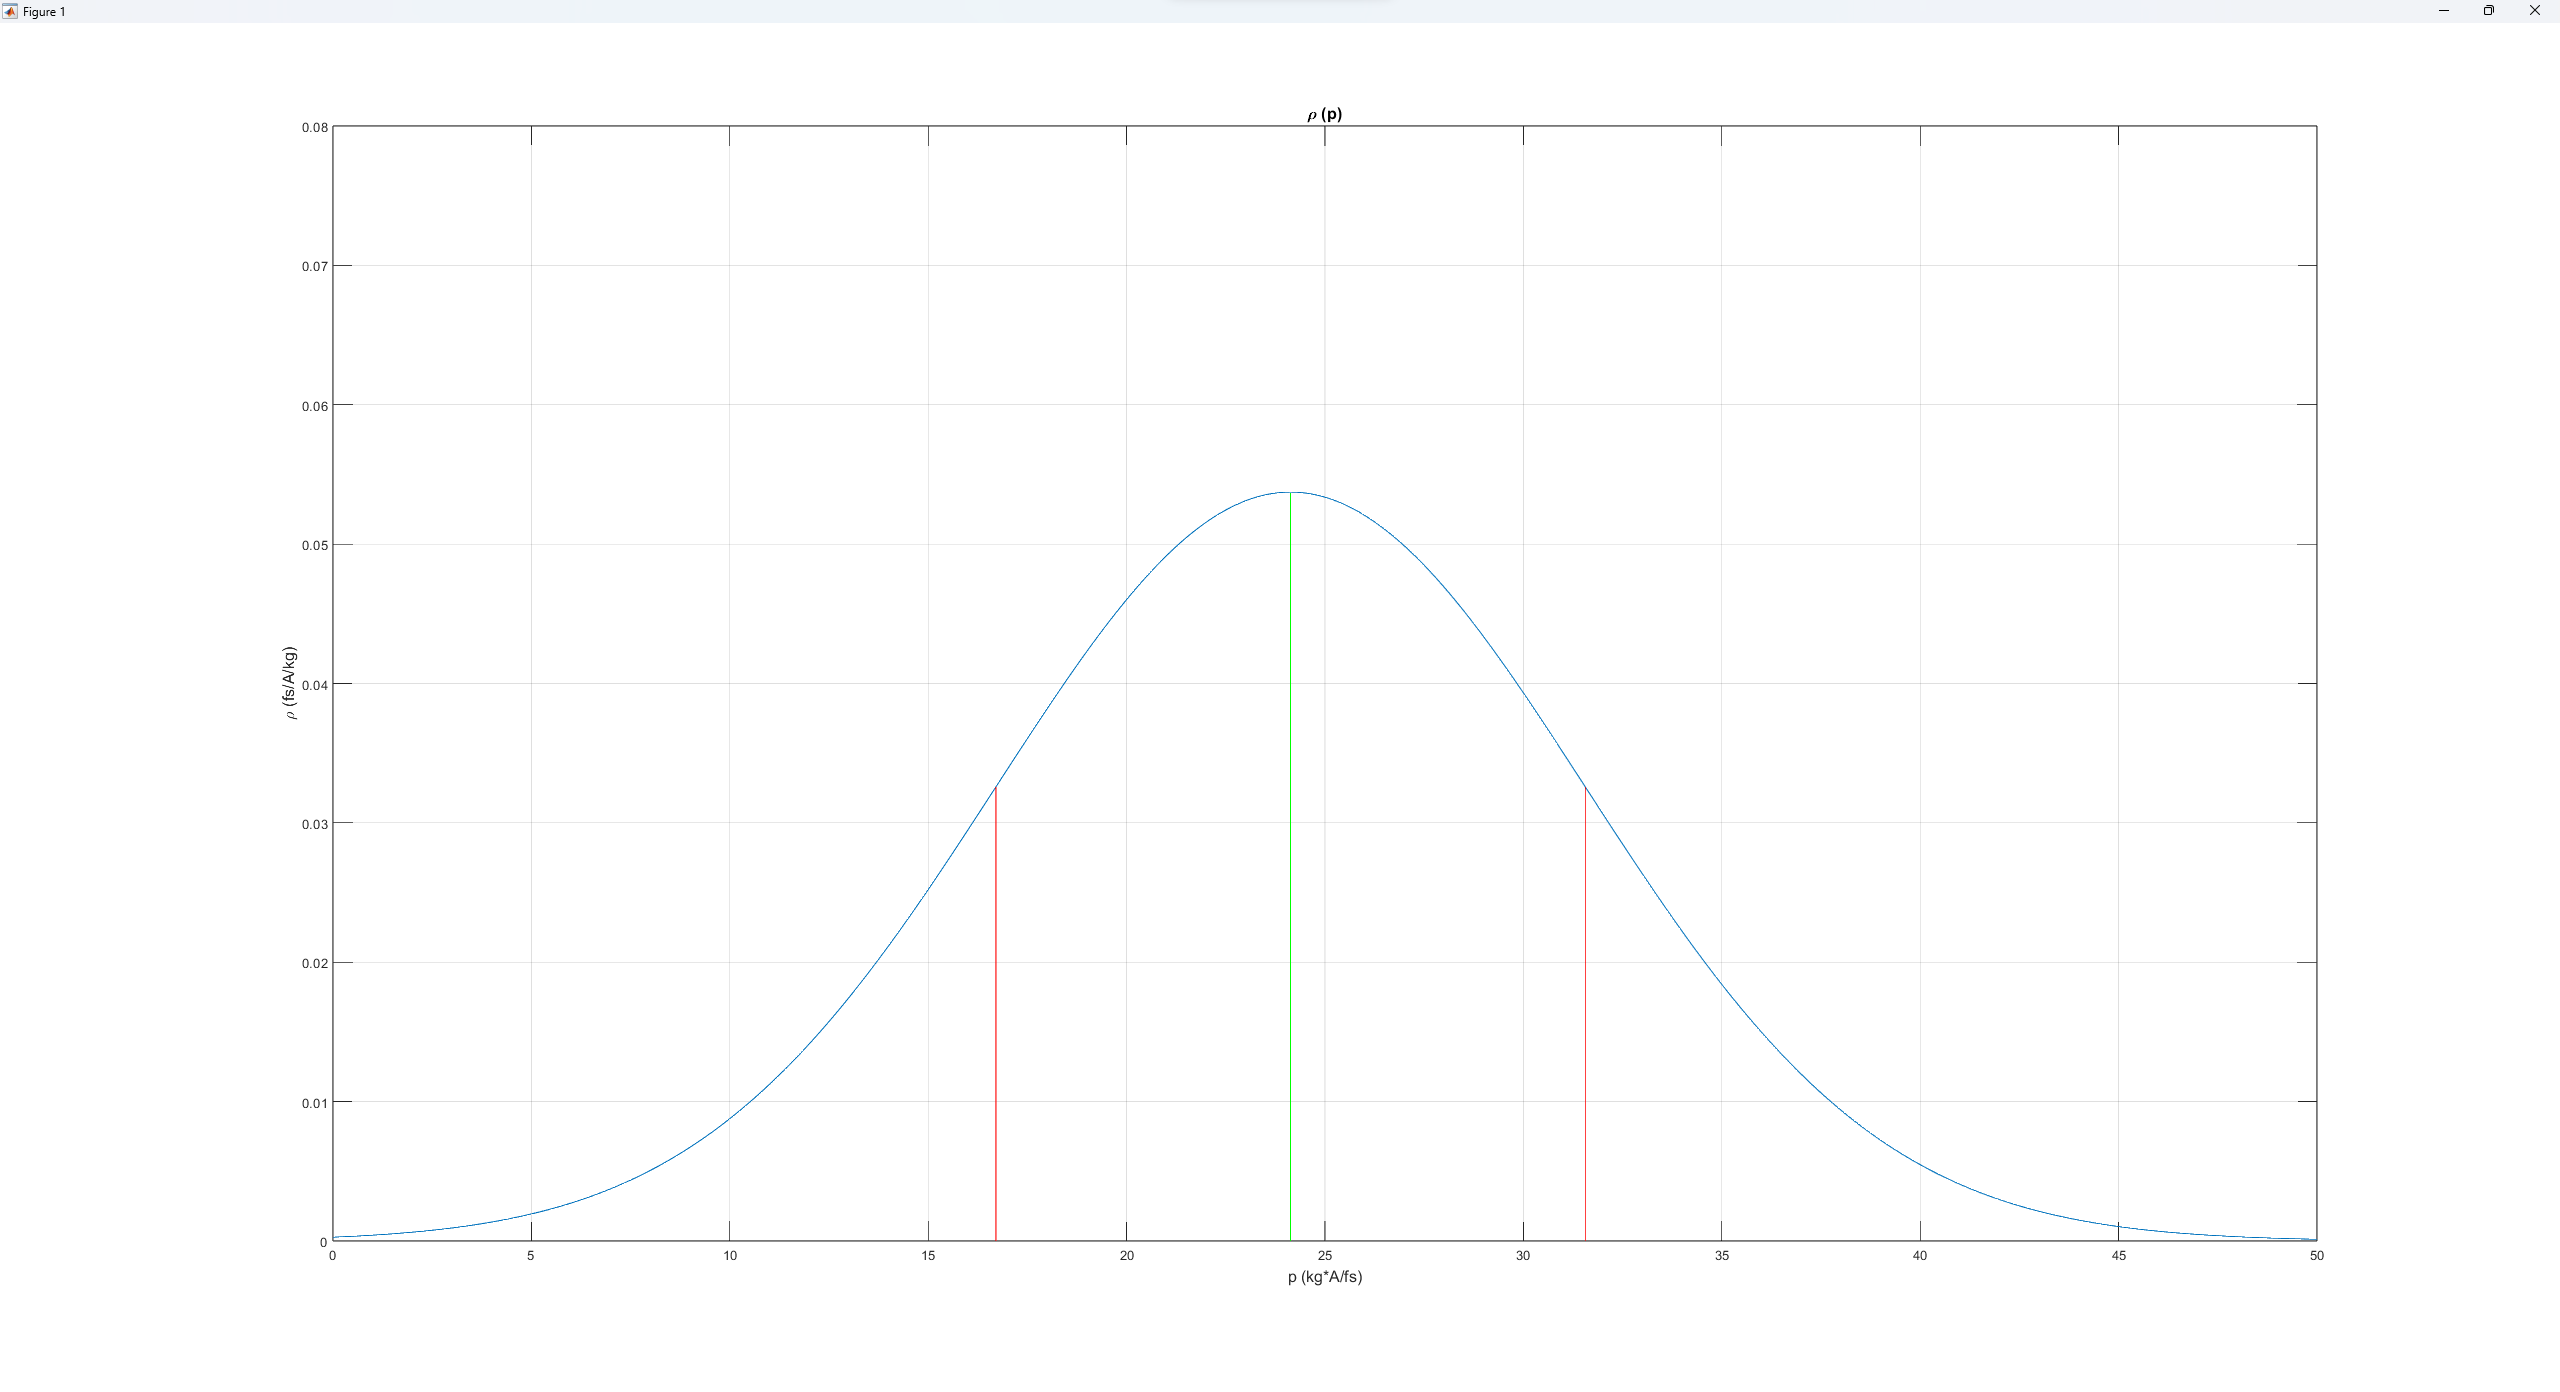
\includegraphics[width=\textwidth]{Lab2qmTask5.png}
\caption{График распределения вероятности по импульсам $\rho(p)$ для $E_0 = 20$ эВ и $d_0 = 1$ Å.}
\label{fig:lab2qmTask5}
\end{figure}
красные линии соответствуют среднеквадратическим отклонениям от $p_0$, рассчитанным по формуле
\begin{equation}
	\sigma_p = \frac{\hbar}{d_0\sqrt{2}}
	\label{eq:root mean square deviation of momentum}
\end{equation} 
в свою очередь вероятность иметь импульс в интервале 
$[p_0 - \sigma_p, p_0 + \sigma_p]$ можно найти по формуле
\begin{equation}
	P\{p_0 - \sigma_p \leq p \leq p_0 + \sigma_p\} = \int\limits_{p_0 - \sigma_p}^{p_0 + \sigma_p} \rho(p) dp = \int\limits_{p_0 - \sigma_p}^{p_0 + \sigma_p} \frac{d_0}{\hbar\sqrt{\pi}} e^{-\frac{(p-p_0)^2d_0^2}{\hbar^2}} dp
	\label{eq:probability}
\end{equation}
используя формулы (\ref{eq:impulse}), (\ref{eq:root mean square deviation of momentum}) и 
(\ref{eq:probability}) найдём величины для параметров системы:
\begin{equation*}
	p_0 = \sqrt{2m_{e^-}E_0} = \sqrt{2\cdot 9.1\cdot 10^{-31}\cdot 20\cdot 1.6\cdot 10^{-19}} \approx 24.16 \times 10^{-30} \text{ кг}\cdot\text{Å/фс}
\end{equation*}
\begin{equation*}
	\sigma_p = \frac{\hbar}{d_0\sqrt{2}} = \frac{1.05\cdot 10^{-34}}{1\cdot 10^{-10}\sqrt{2}} \approx 7.43 \times 10^{-30} \text{ кг}\cdot\text{Å/фс}
\end{equation*}
\begin{equation*}
\begin{aligned}
	P\{p_0 - \sigma_p \leq p \leq p_0 + \sigma_p\} &= \int\limits_{p_0 - \sigma_p}^{p_0 + \sigma_p} \rho(p) dp 
		= \int\limits_{p_0 - \sigma_p}^{p_0 + \sigma_p} \frac{d_0}{\hbar\sqrt{\pi}} e^{-\frac{(p-p_0)^2d_0^2}{\hbar^2}} dp = \\
		&= \left|\begin{matrix}
			u = \frac{(p-p_0)d_0}{\hbar}	& u_\text{в} = \frac{\sigma_pd_0}{\hbar} \\
			du = \frac{d_0}{\hbar}dp 		& u_\text{н} = -\frac{\sigma_pd_0}{\hbar}
		\end{matrix}\right| = \frac{1}{\sqrt{\pi}}\int\limits_{-\frac{\sigma_pd_0}{\hbar}}^{\frac{\sigma_pd_0}{\hbar}}  e^{-u^2} du
\end{aligned}
\end{equation*}

Разложим функцию в ряд Тейлора, так как функция $e^{-u^2}$ является чётной, то промежуток интегрирования симметричный, соответственно разложить логично в окрестноти нуля, тогда
\begin{equation*}
\begin{aligned}
	e^{-u^2} &= 1 - u^2 + \frac{u^4}{2} - \frac{u^6}{6} + \frac{u^8}{24} \pm \frac{e^{-\xi^2}}{120}u^{10}\quad\xi\in[0,\, u] \\
	\Delta(e^{-u^2})_{max} &= \frac{u^{10}}{120}
\end{aligned}
\end{equation*}

Так как промежуток интегрирования симметричный, то можно сократить промежуток интегрирования до $[0, \frac{\sigma_pd_0}{\hbar}]$, тогда
\begin{equation*}
\begin{aligned}
	P\{p_0 - \sigma_p \leq p \leq p_0 + \sigma_p\} &= \frac{2}{\sqrt{\pi}}\int\limits_{0}^{\frac{\sigma_pd_0}{\hbar}}  e^{-u^2} du = \\
	&= \frac{2}{\sqrt{\pi}}\int\limits_{0}^{\frac{\sigma_pd_0}{\hbar}}  \left(1 - u^2 + \frac{u^4}{2} - \frac{u^6}{6} + \frac{u^8}{24}\right) du \pm \frac{2}{\sqrt{\pi}}\int\limits_{0}^{\frac{\sigma_pd_0}{\hbar}}  \frac{u^{10}}{120} du = \\
	&= \frac{2}{\sqrt{\pi}}\left(\frac{\sigma_pd_0}{\hbar} - \frac{(\sigma_pd_0)^3}{3\hbar^3} + \frac{(\sigma_pd_0)^5}{10\hbar^5} - \frac{(\sigma_pd_0)^7}{42\hbar^7} + \frac{(\sigma_pd_0)^9}{216\hbar^9}\right) \pm \\ \pm \frac{2}{\sqrt{\pi}}\cdot \frac{(\sigma_pd_0)^{11}}{1320\hbar^{11}} = 0.68271 \pm 0.00002
\end{aligned}
\end{equation*}

Используем условие нормировки функции распределения вероятности по импульсам 
\begin{equation*}
	\frac{1}{\sqrt{\pi}}\int\limits_{-\infty}^{+\infty}  e^{-u^2} du = 1
\end{equation*}

Значит 

\begin{equation*}
	\begin{aligned}
	P\{-\infty < p_0 - \sigma_p \leq p \leq p_0 + \sigma_p < +\infty\} = 1 - P\{p_0 - \sigma_p \leq p \leq p_0 + \sigma_p\} = \\ 
	= 1 - (0.68271 \pm 0.00002) = 0.31729 \pm 0.00002 
	\end{aligned}
\end{equation*}
\begin{equation*}
	\begin{aligned}
	P\{-\infty < p \leq p_0 - \sigma_p\} &= P\{p_0 + \sigma_p \le p < +\infty\} = \frac{P\{-\infty < p_0 - \sigma_p \leq p \leq p_0 + \sigma_p < +\infty\}}{2} = \\
	&= \frac{0.31729 \pm 0.00002}{2} = 0.158645 \pm 0.00001
	\end{aligned}
\end{equation*}

Зафиксируем результаты в Таблице \ref{tab:lab2qmTask5part1}.

\begin{center}
	\begin{table}[h]
		\noindent
		\begin{tabularx}{\textwidth}{|>{\centering\arraybackslash}X|>{\centering\arraybackslash}X|>{\centering\arraybackslash}X|>{\centering\arraybackslash}X|>{\centering\arraybackslash}X|>{\centering\arraybackslash}X|>{\centering\arraybackslash}X|}
		\hline
		$p_0$, \text{кг·Å/фс} & $\sigma_p$, \text{кг·Å/фс} & $P\{-\infty < p \leq p_0 - \sigma_p\}$ & $P\{p_0 - \sigma_p \leq p \leq p_0 + \sigma_p\}$ & $P\{p_0 + \sigma_p \leq p < +\infty\}$ \\
		\hline
		$24.16 \times 10^{-30}$ & $7.43 \times 10^{-30}$ & $0.158645 \pm 0.00001$ & $0.68271 \pm 0.00002$ & $0.158645 \pm 0.00001$ \\
		\hline
		\end{tabularx}
		\caption{Результаты расчёта параметров распределения вероятности по импульсам для $E_0 = 20$ эВ и $d_0 = 1$ Å.}
		\label{tab:lab2qmTask5part1}
	\end{table}
\end{center}

Неопределённость координаты в отличие от неопределённости импульса изменяется во времени, 
согласно формуле
\begin{equation}
	\sigma_x(t) = \frac{d(t)}{\sqrt{2}}
\end{equation}

Воспользуемся данными из Таблицы \ref{tab:lab2qmTask2} для нахождения $\sigma_x(t)$ 
\begin{equation*}
	\begin{aligned}
		\frac{2\sigma_p\sigma_x(0.2165)}{\hbar} &= \frac{d(0.2165)}{\sqrt{2}}\frac{2\sigma_p}{\hbar} = \frac{2.6908}{\sqrt{2}} \frac{2\cdot 7.43}{1.05} \frac{10^{-35}}{10^{-34}} = 2.692 \\
		\frac{2\sigma_p\sigma_x(0.411)}{\hbar} &= \frac{d(0.411)}{\sqrt{2}}\frac{2\sigma_p}{\hbar} = \frac{4.8466}{\sqrt{2}} \frac{2\cdot 7.43}{1.05} \frac{10^{-35}}{10^{-34}} = 4.847 \\
		\frac{2\sigma_p\sigma_x(0.611)}{\hbar} &= \frac{d(0.611)}{\sqrt{2}}\frac{2\sigma_p}{\hbar} = \frac{7.1206}{\sqrt{2}} \frac{2\cdot 7.43}{1.05} \frac{10^{-35}}{10^{-34}} = 7.124 \\
		\frac{2\sigma_p\sigma_x(0.808)}{\hbar} &= \frac{d(0.808)}{\sqrt{2}}\frac{2\sigma_p}{\hbar} = \frac{9.3766}{\sqrt{2}} \frac{2\cdot 7.43}{1.05} \frac{10^{-35}}{10^{-34}} = 9.382 \\
		\frac{2\sigma_p\sigma_x(1.2075)}{\hbar} &= \frac{d(1.2075)}{\sqrt{2}}\frac{2\sigma_p}{\hbar} = \frac{13.9685}{\sqrt{2}} \frac{2\cdot 7.43}{1.05} \frac{10^{-35}}{10^{-34}} = 13.972
	\end{aligned}
\end{equation*}

\begin{center}
	\begin{table}[h]
		\noindent
		\begin{tabularx}{\textwidth}{|>{\centering\arraybackslash}X|>{\centering\arraybackslash}X|>{\centering\arraybackslash}X|>{\centering\arraybackslash}X|>{\centering\arraybackslash}X|>{\centering\arraybackslash}X|}
		\hline
		 & $1$ & $2$ & $3$ & $4$ & $5$ \\
		\hline
		$t$, фс & $0.2165$ & $0.411$ & $0.611$ & $0.808$ & $1.2075$ \\
		\hline
		$\sigma_p\sigma_x(t)\geq\frac{\hbar}{2}$ & $2.692>1$ & $4.847>1$ & $7.124>1$ & $9.382>1$ & $13.972>1$ \\
		\hline
		\end{tabularx}
		\caption{Наглядное подтверждение роста неопределённости координаты во времени
		и соответствующего роста выражения $\sigma_p\sigma_x(t)$ из неопределённости Гейзенберга.}
		\label{tab:lab2qmTask5part2}
	\end{table}
\end{center}

\end{document}